\documentclass[12pt,a4paper]{article}

% Margins.
\setlength{\oddsidemargin}{0in}
\setlength{\evensidemargin}{0in}
\setlength{\headheight}{12pt}
\setlength{\headsep}{42pt}
\setlength{\topmargin}{-54pt}
\setlength{\textwidth}{6.5in}
\setlength{\textheight}{10in}

\usepackage{amsmath}
\usepackage{float}
\usepackage{graphicx}
\usepackage[hyphens]{url}
\usepackage{hyperref}	% Clickable links to figures, references and urls.
\usepackage{datetime}
\usepackage{longtable}
\usepackage{subfigure}

% Links direct to top of figures.
\usepackage[all]{hypcap}

% Drawing.
\usepackage{pgf}
\usepackage{tikz}

% Listings for formatting code.
\usepackage{listings}
\usepackage{textcomp}
% General options.+++
\lstset{breaklines=true, basicstyle=\small\ttfamily, tabsize=4, numbers=left, stepnumber=1, frame=single, showstringspaces=false, upquote=true}
% C++ specific high-lighting. Comments are 50/50 shades of green/black and strings coloured with 60/40 red/black mixture.
\lstset{language=[ISO]C++, commentstyle=\color{green!50!black}, keywordstyle=\color{blue}, stringstyle=\color{red!60!black}}

%opening
\title{\vspace{-3cm}Physics for Engineers\\Class 43\\Electromagnetic Waves}
\author{Attique Dawood}
\date{May 05, 2014\\[0.2cm] Last Modified: \today, \currenttime}
\begin{document}
\maketitle
\section{Announcements}
\begin{itemize}
\item None.
\end{itemize}
\section{What Exactly is a Wave?}
A wave is some \textit{disturbance} or \textit{pattern} that \textit{moves}. An example of wave is when you fix one end of a string and shake the other end then the string moves up and down. You see a sinusoidal patterns moving on the string. Another example is that of water waves. Just drop something still water and water ripples will start moving from the point of impact. The first example wave was made of string (being moved in a certain pattern). The water waves are made of particles of water.
\section{Electromagnetic Wave}
Just like any other physical wave we have electromagnetic waves or EM waves for short. EM waves are composed of disturbances in electric and magnetic field. When electric and magnetic fields change together in a certain pattern then they make up EM wave.
\section{Electromagnetic Radiation}
EM waves are produced as a result of EM \textit{radiation}. \textbf{EM radiations are produced when a charge is accelerated}. Radiations depend on the acceleration. If there is little acceleration then there are no radiations or so little that they are barely noticeable.

Making a moving object suddenly stop completely and then make it move in opposite direction requires a lot of acceleration (actually deceleration). Consequently, the best way to produce EM radiation is to take an electron (or charge) and shake it (very) violently. You want to relieve the electron of its electric field; just like if you drop your handkerchief you shake it to remove dirt. But how can you shake a charge to near--relativistic levels? The answer is AC sources that can produce frequencies in the MHz range can easily produce EM radiation. TV antennas, mobile phones, laptops etc. do that all the time.
\section{Characteristics of EM Waves}
When studying EM waves it is best to consider waves with a sinusoidal pattern because these can be easily manipulated mathematically. It is important to note that waves are functions of both space and time ($f(x,t)$). This is to say that if you keep time fixed then you'll get one pattern. If you take a point and observe the wave in time then you'll get another pattern. A Matlab demo demonstrates such a wave in real--time.

\textbf{Wavelength} is the distance between two crests or troughs. It is the \textit{physical length} of one complete cycle of wave. \textbf{Time period} is the \textit{temporal length} of one complete cycle, the time it takes to complete one cycle. \textbf{Frequency} is the inverse of time period and gives number of temporal cycles per second. Frequency, wavelength and speed of wave are related by the formula
\begin{equation}
v=f\lambda.
\end{equation}
In free space $v=c$. Light is also an EM wave with a certain frequency.

\section{Exercises}
\noindent\textbf{Question 1} Run \verb|Drude_1D_DNG_Transmission_Coefficient.m| file in Matlab. Determine frequency, time period and wavelength of the wave.\\
%\begin{figure}[H]
%\centering
%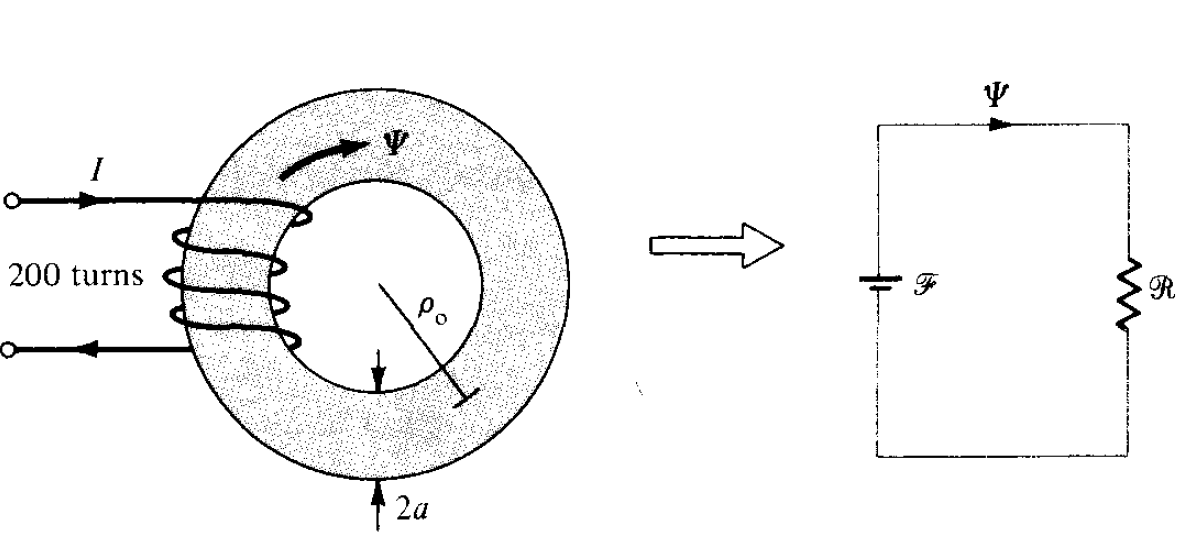
\includegraphics[scale=0.4]{Figure8-26S.png}
%\caption{Toroid and equivalent magnetic circuit.}
%\label{Toroid-and-equivalent-circuit}
%\end{figure}
%\nocite{*}
\bibliographystyle{plain}
\bibliography{PhysicsRef}
\end{document}
